\chapter*{Analisi del Rumore In Ingresso}\label{cap:rumore}

Il primo passo per analizzare il segnale audio in ingresso è quello di valutare il rumore presente durante le operazioni di registrazione e conversione analogico-digitale del segnale effettuate dalla scheda audio. 

Per valutare tale fenomeno sono state realizzate diverse registrazioni in assenza di segnale utile. 
Per evitare che l'analisi del rumore venisse influenzata da effetti temporanei che concentrassero la maggior parte dell'energia in particolari frequenze, le misure sono state effettuate in diversi momenti della giornata.
Inoltre, dal momento che non si può escludere la presenza di disturbi esterni casuali concentrati in particolari frequenze, si è cercato di isolare il più possibile la zona di registrazione da tali disturbi, in modo tale da mantenere l'intensità di questi suoni inferiore rispetto a quella del segnale utile.
 
La figura \ref{fig:rumore} rispecchia l'andamento del rumore in condizioni standard, cioè in assenza di rumori a intensità molto elevate vicini allo strumento di registrazione. 
I parametri di registrazione sono quelli utilizzati per la registrazione del segnale e verranno descritti nel capitolo successivo.
Lo spettro mostrato è tipico del rumore rosa. 
Le intensità della componente continua, in particolare, risulta essere molto elevata.

Si discuterà del filtro utilizzato per ridurre il rumore nel capitolo \todo{inserire riferimento al capitolo}.

	\begin{figure}[h]
	  \begin{center} 
	    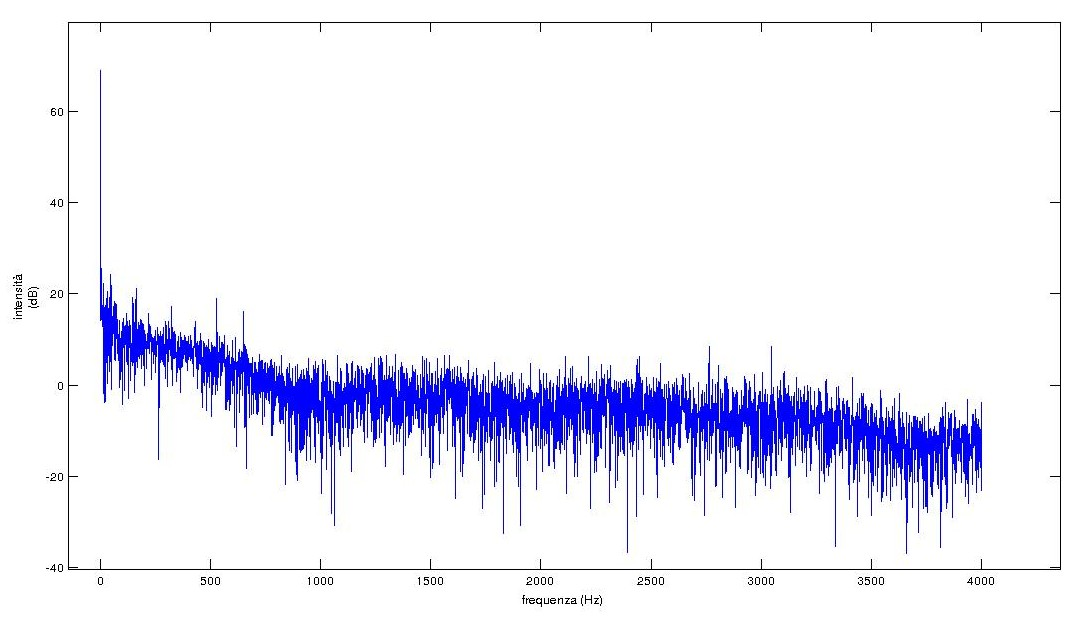
\includegraphics[width=\textwidth*\real{0.9}]{images/ch_02/spettro_rumore.jpg}
	  \end{center} 
	  \caption{\textit{Rumore di registrazione}}  
	  \label{fig:rumore}
	\end{figure}



